\documentclass{beamer}
\usetheme{ensam}
\usepackage{pgfplots}
\usepackage{subcaption}
\usepackage{acronym}
\usepackage{tikz}
\usepackage{pgf-pie}
\usetikzlibrary{calc}
\usepackage{amsmath}
\usepackage {algorithmic}
\usepackage{algorithm}
\usepackage{eqparbox}
\usepackage[font=scriptsize]{caption}
\usetikzlibrary{bayesnet,positioning,calc}
\tikzstyle{obs} = [latent,fill=lightBlue]
\tikzstyle{default}=[draw=sexyRed,thick,rounded corners,text width=0.5in,font=\scriptsize,align=center]
\usepgfplotslibrary{colorbrewer}
\definecolor{ForestGreen}{RGB}{34,139,34}
\newcommand{\comment}[1]{\textcolor{ForestGreen}{#1}}
%algorithmic comment
\renewcommand\algorithmiccomment[1]{%
  \hfill\comment{\#\scriptsize\eqparbox{COMMENT}{#1}}%
}
\renewcommand{\algorithmicrequire}{\textbf{Input:}}
\renewcommand{\algorithmicensure}{\textbf{Output:}}
\title{Ensembles et Applications}
\author{\underline{A.Belcaid}}
\institute{\small École Nationale des Sciences Appliqués.} 


% Customzation {{{ %
% }}} Customzation %

%tikz bayesian theme
\usetikzlibrary{bayesnet,positioning,calc}
\tikzstyle{obs} = [latent,fill=lightBlue]
\tikzstyle{default}=[draw=sexyRed,thick,rounded corners,text width=0.5in,font=\scriptsize,align=center]
\DeclareMathOperator{\argmin}{argmin}

\pgfplotsset{every tick label/.append style={font=\tiny}}





% add bibliography
\date{19 octobre 2020}

\begin{document}
\maketitle

% Logistics {{{
% Appercu du cours {{{ %
\begin{frame}[t]
  \frametitle{Apperçu du cours}
  \begin{enumerate}
    \item Ensembles et Applications.
      \begin{itemize}
        \scriptsize
        \item Ensembles.
        \item Applications.
        \item Injection/Surjection/Bijection.
        \item Ensembles finis.
        \item Relations d'équivalence.
      \end{itemize}
    \item Nombres Complexe
      \begin{itemize}
        \scriptsize
        \item Définition.
        \item Equation de second ordre.
        \item Trigonométrie.
        \item Relation avec la géométrie.
      \end{itemize}
    \item Théorie de groupes
      \begin{itemize}
        \scriptsize
        \item Groupe.
        \item Sous groupes.
        \item Morphisme de groupe.
        \item Groupe de permutation.
      \end{itemize}
    \item Polynômes
      \begin{itemize}
        \scriptsize
        \item Définition.
        \item Arithmétique sur les polynômes.
        \item Racine de polynômes.
        \item Fractions rationnelles.
      \end{itemize}
  \end{enumerate} 
\end{frame}
% }}} Appercu du cours %
% Livre de référence {{{1 %
\begin{frame}[t]
  \frametitle{Livre de Référence}
  \vspace*{1cm}
  \centering
  \begin{tabular}{cc}
    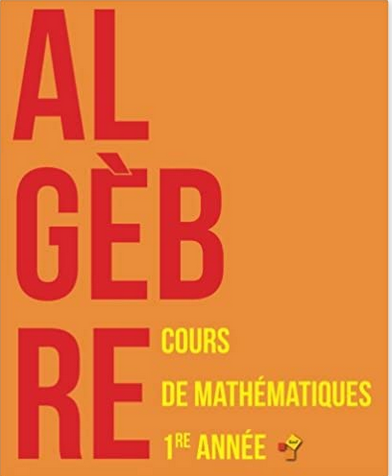
\includegraphics[width=4cm, height=5cm]{./book1.png} &
    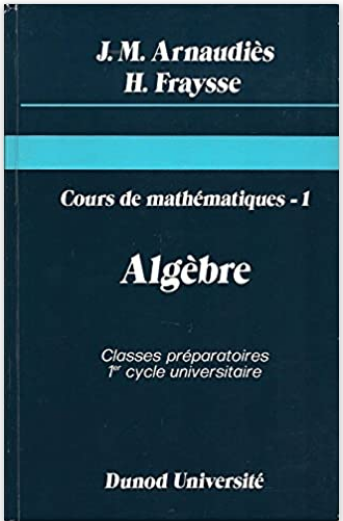
\includegraphics[width=4cm, height=5cm]{./book2.png}  
  \end{tabular}
\end{frame}
% }}} Logistics %
% Grading {{{ %
\begin{frame}[t]
  \frametitle{Note du module}
  \begin{figure}[htpb]
    \centering
    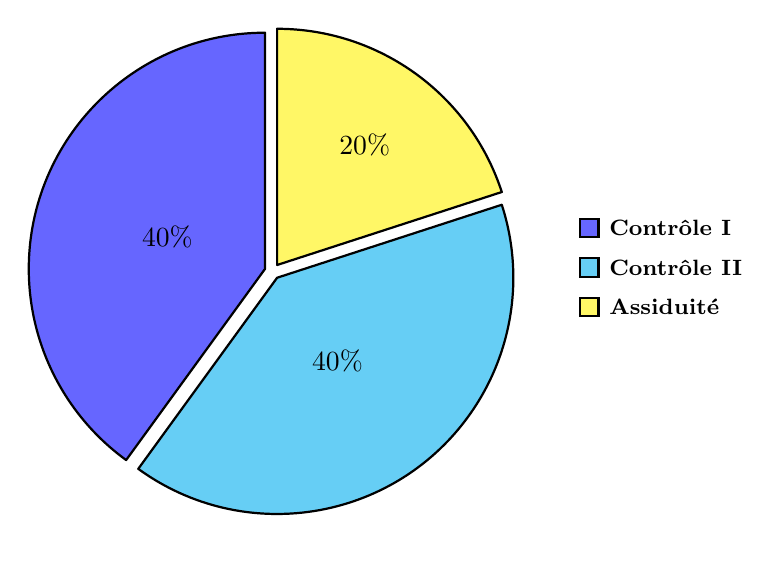
\begin{tikzpicture}
      \pie[rotate=90, explode=0.1, text=legend]{40/\textbf{Contrôle I}, 40/
        \textbf{Contrôle II} , 20/
      \textbf{Assiduité} }
    \end{tikzpicture}
  \end{figure} 
\end{frame}
% }}} Grading %

% Piazza {{{ %
% Platforme de discusssion {{{ 
\begin{frame}[t]
  \frametitle{Platforme de discussion}
  \begin{figure}[htpb]
    \centering
    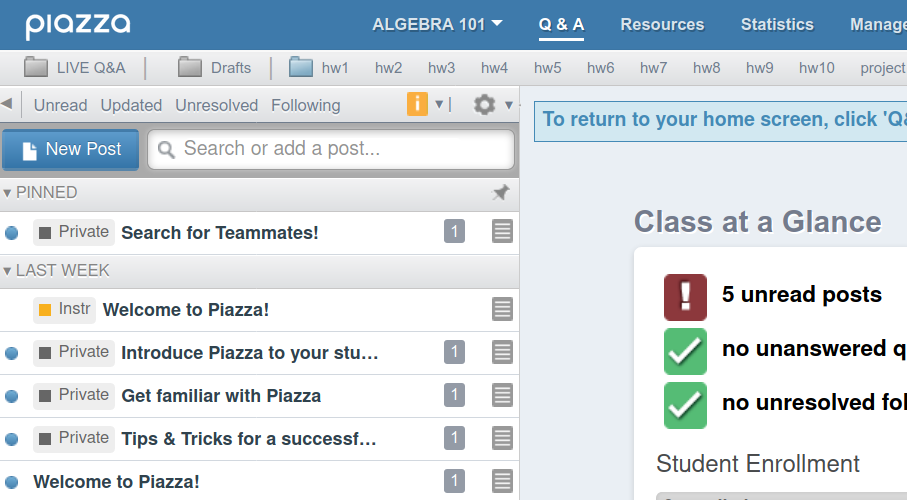
\includegraphics[width=0.8\linewidth]{./piazza.png}
    \caption{Plateforme de discussion}%
    \label{fig:./piazza}
  \end{figure} 
    \centering
    \Large
    \alert{https://piazza.com/class/l96sp61sjyj6lr}
\end{frame}
% }}} Platforme de discusssion %
% }}} Piazza %
%}}}




% Définition {{{ %
% Exemples a priori {{{ %
\begin{frame}[t]
  \frametitle{Ensembles}
  {\small
     Dans votre apprentissage de mathématiques, vous avez utiliser les
      ensembles suivants:
    }

  \begin{enumerate}
    \item Ensemble des nombres \alert{\textbf{entiers naturels}}: $$\mathbb{N} =
      \{0,1,2,3,\ldots\}$$
    \item Ensemble des nombres \alert{\textbf{entiers relatifs}}: $$\mathbb{Z} =
      \{\ldots, -2, -1, 0, 1, 2, \ldots\}$$
    \item Ensemble des nombre \alert{\textbf{rationnels}}:
      $$
      \mathbb{Q} = \{\frac{p}{q}\;|\; p\in\mathbb{Z}, q\in
      \mathbb{N}\backslash\{0\}\}
      $$
    \item Ensemble des \alert{\textbf{réels}} $\mathbb{R}$ comme $\sqrt{2}$, $\pi$, et
      $\log(2)$.
    \item Finalement l'ensemble des nombres \alert{\textbf{complexes}}
      $\mathbb{C}$.
  \end{enumerate}
\end{frame}
% }}} Exemples %

% Définition Ensemble {{{ %
\begin{frame}[<+->]
  \frametitle{1. Ensembles}
  \begin{block}{Définition}
    \scriptsize

    \begin{itemize}
      \item Un \textbf{\alert{ensemble}} est une collection d'objets mathématiques (\textbf{éléments})
    rassemblées selon une ou plusieurs \textbf{propriétés}
    mathématiques.\\[4pt]

  \item Ces propriétés seront suffisantes pour \textbf{affirmer}  si un élément
    \textbf{appartient} a cet ensemble.
\end{itemize}
  \end{block}
\begin{block}{Exemples}
  \begin{itemize}
    \scriptsize
    \item Ensemble des couleurs $\{\text{rouge}, \text{vert}, \text{bleu}\}$.
    \item Ensemble des nombres \textbf{pairs}:
      \begin{equation*}
        P = \{ n \in \mathbb{N}\;|\; 2 \text{ divise } n\}
      \end{equation*}
    \item 
      \begin{equation*}
        \{x\in\mathbb{R}\;|\; \vert x - 2 \vert < 1\}
      \end{equation*}
    \item 
      \begin{equation*}
        \{x\in\mathbb{R}\;|\; x^2 - 1 = 0\} 
      \end{equation*}
  \end{itemize}
\end{block}
\end{frame}
% }}} Définition Ensemble %
% Ensemble vide et appartenance {{{ %
\begin{frame}[<+->]
  \frametitle{2.1 Appartenance}
  
  \begin{block}{Appartenance}
    \scriptsize
    \begin{itemize}
      \item 
   Si un en élément $x$ appartient à un ensemble $E$. On écrit:
   \begin{equation}
     x \in E
   \end{equation}
 \item Dans le cas contraire:
   \begin{equation}
     x \not\in E
   \end{equation}
 \end{itemize}
  \end{block}
  \begin{block}{Exemple}
   \scriptsize 
   \begin{columns}
     \column{0.3\textwidth}
      $ 2 \in \mathbb{N}$.
     $ -2 \not\in \mathbb{N}$.
     $ \sqrt{2} \notin \mathbb{Q}$.
  \end{columns}
  \end{block}

  \begin{block}{Ensemble vide}
    \scriptsize
    Un ensemble \textbf{particulier}  est l'ensemble \textbf{\alert{vide}} note
    $\alert{\mathbf{\emptyset}}$ et qui ne contient aucun élément.
    
  \end{block}
\end{frame}
% }}} Ensemble vide et appartenance %
% }}} Définition %
% Opérations {{{ %
% Inclusion {{{ %
\begin{frame}[<+->]
  \frametitle{2. Relations entre ensemble}
  \small

  \begin{columns}
    \begin{column}{0.7\textwidth}
      
 \begin{block}{Inclusion}
   On note $\mathbf{ E \subset F}$ si \alert{tous} les éléments de $E$ sont dans
   $F$.

   \begin{equation}
    E \subset F \iff \forall x\in E \quad x\in E \implies x\in F
   \end{equation}
 \end{block} 
 \begin{itemize}
   \item On dit aussi que $E$ est un \textbf{\alert{sous ensemble}} ou une
     \textbf{\alert{partie}}  de $F$.
 \end{itemize}
    \end{column}
    \begin{column}{0.3\textwidth}
     \begin{figure}[htpb]
     \begin{center}
     \begin{tikzpicture}
       \draw[draw=sexyRed, thick ] (-0.5,0) ellipse (1.5cm and 0.8cm); 
       \node at (-2.3, 0) {$F$};
       \draw[draw=lightBlue, thick ] (0,0) ellipse (0.5cm and 0.6cm); 
       \node at (-0.6, 0) {$E$};
     \end{tikzpicture}
     \end{center}
     \caption{Inclusion}%
     \label{fig:}
     \end{figure}
      
    \end{column}
  \end{columns}

  \begin{columns}
    \begin{column}{0.7\textwidth}
 \begin{block}{Négation}
  \begin{equation}
    E \not\subset F \iff \pause (\exists x \in E) \text{ tel que } x\not\in F 
  \end{equation} 
 \end{block}
    \end{column}
    \begin{column}{0.3\textwidth}
     \begin{center}
     \begin{tikzpicture}
       \draw[draw=sexyRed, thick ] (-0.5,0) ellipse (1.5cm and 0.8cm); 
       \node at (-2.3, 0) {$F$};
       \draw[draw=lightBlue, thick ] (0.7,0.4) ellipse (0.5cm and 0.6cm); 
       \node at (0.7, 0.9) {$E$};
     \end{tikzpicture}
     \end{center}
      
    \end{column}
  \end{columns}
\end{frame}
% }}} Inclusion %

% Egalité {{{ %
\begin{frame}
  \small
  \frametitle{Égalité et Complémentaire}
 \begin{block}{Égalité}
  \begin{equation}
    E = F \iff  (E \subset F)\; \text{et}\; (F \subset E)
  \end{equation} 
 \end{block} 
 \pause
\begin{columns}
  \begin{column}{0.7\textwidth}
    
    \begin{block}{Complémentaire}
      Si $A \subset E$, on note son \textbf{\alert{complémentaire}} $\mathtt{C}_E A$
       l'ensemble:

       \begin{equation}
         \mathtt{C}_E A = \left\{ x \in E \;|\; x \not\in A \right\}
       \end{equation}
    \end{block}
  \end{column}
  \begin{column}{0.3\textwidth}
    
     \begin{tikzpicture}
       \draw[draw=black, thick, fill=sexyRed!40 ] (-0.5,0) ellipse (1.5cm and 0.8cm); 
       \node at (-2.1, 0) {$E$};
       \draw[draw=black, thick, fill=lightBlue!80 ] (0,0) ellipse (0.5cm and 0.6cm); 
       \node at (0, 0) {$\small A$};
       \node at (-1.5, 0) {${\small \mathtt{C}_E A}$};
     \end{tikzpicture}
  \end{column}
\end{columns}
\begin{itemize}
  \item Dans la littérature on trouve aussi les notations  $A^c$, $\overline{A}$
    ou $ E\backslash A$.
\end{itemize}
\end{frame}
% }}} Egalité %
% Union Intersection {{{ %
\begin{frame}[t]
  \frametitle{Union Intersection}
  
  \small
  \begin{columns}
    \begin{column}{0.7\textwidth}
     \begin{block}{Union}
       Pour deux ensembles $A$ et $B \subset E$, On note \textbf{\alert{l'union}} $A\cup
         B$:
         \begin{equation}
           A\cup B = \left\{ x \in E\;|\; x\in A\text{ \textbf{ou} } x\in B\right\} 
         \end{equation}
     \end{block} 
     {\scriptsize
     On doit mentionner que le \textbf{ou} n'est pas exclusive, i.e x peut
   appartenir ou deux ensembles en même temps.}
    \end{column}
    \begin{column}{0.3\textwidth}
     \begin{center}
       
     \begin{tikzpicture}
       \draw[very  thick] (-0.5,0) ellipse (1cm and 0.6cm); 
       \node at (-0.5, 0.8) {$A$};
       \draw[ very thick ] (0.5,0) ellipse (1cm and 0.6cm); 

       \fill[ sexyRed!60] (-0.5,0) ellipse (1cm and 0.6cm); 
       \fill[sexyRed!60 ] (0.5,0) ellipse (1cm and 0.6cm); 
       \node at (0.5, 0.8) {$B$};
       \node at (0, 0.2) {$A \cup B $};

     \end{tikzpicture}
     \end{center}
    \end{column}
  \end{columns}

  \vspace*{1cm}
  \begin{columns}
    \begin{column}{0.7\textwidth}
     \begin{block}{Intersection}
       Pour deux ensembles $A$ et $B \subset E$, On note
       \textbf{\alert{l'intersection}} $A\cap
         B$:
         \begin{equation}
           A\cap B = \left\{ x \in E\;|\; x\in A\text{ \textbf{et} } x\in B\right\} 
         \end{equation}
     \end{block} 
    \end{column}
    \begin{column}{0.3\textwidth}
     \begin{center}
       
     \begin{tikzpicture}
       \draw[very  thick] (-0.5,0) ellipse (1cm and 0.6cm); 
       \node at (-0.5, 0.8) {$A$};
       \draw[ very thick ] (0.5,0) ellipse (1cm and 0.6cm); 

       \fill[lightBlue] (-0.5,0) ellipse (1cm and 0.6cm); 
       \fill[lightBlue ] (0.5,0) ellipse (1cm and 0.6cm); 
       \node at (0.5, 0.8) {$B$};
       \draw[fill=white,even odd rule] (-0.5,0) ellipse (1cm and 0.6cm)
         (0.5,0) ellipse (1cm and 0.6cm);
       \node at (0,0) {\scriptsize$A\cap B$};

     \end{tikzpicture}
     \end{center}
    \end{column}
  \end{columns}

    {\small Si $A\cap B= \emptyset$, on dit que $A$ et $B$ sont
    \alert{\textbf{disjoints}}}
\end{frame}
% }}} Union Intersection %
%  Différence {{{ %
\begin{frame}[t]
  \frametitle{ Différence}
  \small
  \begin{columns}
    \begin{column}{0.7\textwidth}
     \begin{block}{Différence}
       Pour deux ensembles $A$ et $B \subset E$, On note \textbf{\alert{la
       différence}} $A-B$:
         \begin{equation}
           A- B = \left\{ x \in E\;|\; x\in A\text{ \textbf{et} } x\not\in B\right\} 
         \end{equation}
     \end{block} 
    \end{column}
    \begin{column}{0.3\textwidth}
     \begin{center}
       
     \begin{tikzpicture}
       \draw[ thick] (-0.5,0) ellipse (1cm and 0.6cm); 
       \node at (-0.5, 0.8) {$A$};
       \draw[ thick ] (0.5,0) ellipse (1cm and 0.6cm); 
       \fill[ sexyRed!60] (-0.5,0) ellipse (1cm and 0.6cm); 
       \fill[white] (0.5,0) ellipse (1cm and 0.6cm); 
       \node at (0.5, 0.8) {$B$};
       \node at (-0.9, 0.2) {\scriptsize$A - B $};

     \end{tikzpicture}
     \end{center}
    \end{column}
  \end{columns}

  \vspace*{1cm}
  \begin{columns}
    \begin{column}{0.7\textwidth}
     \begin{block}{Différence symmétrique}
       Pour deux ensembles $A$ et $B \subset E$, On note
       \textbf{\alert{la différence symmétrique}} $A\Delta
         B$:
         \begin{equation}
           A\Delta B =  (A\cup B) \  (B\cap A)
         \end{equation}
     \end{block} 
    \end{column}
    \begin{column}{0.3\textwidth}
     \begin{center}
       
     \begin{tikzpicture}
       \draw[very  thick] (-0.5,0) ellipse (1cm and 0.6cm); 
       \node at (-0.5, 0.8) {$A$};
       \draw[ very thick ] (0.5,0) ellipse (1cm and 0.6cm); 

       % \fill[lightBlue] (-0.5,0) ellipse (1cm and 0.6cm); 
       % \fill[wi ] (0.5,0) ellipse (1cm and 0.6cm); 
       \node at (0.5, 0.8) {$B$};
       \draw[fill=lightBlue,even odd rule] (-0.5,0) ellipse (1cm and 0.6cm)
         (0.5,0) ellipse (1cm and 0.6cm);

     \end{tikzpicture}
     \end{center}
    \end{column}
  \end{columns}
\end{frame}
% }}} Union Intersection %
% Exercices rapides {{{ %
\begin{frame}[t]
  \frametitle{Mini Exercices}
 \small 
  \begin{block}{Mini Exercices}
    \begin{enumerate}
      \item Donner l'ensemble $\{1,2,3\}\cup \{3,4,5\}$
      \item Calculer l'ensemble $\{1,2,3\}\cap \{3,4,5\}$
      \item Calculer $\{1,2,3\} - \{3,4,5\}$.
      \item Donner $\{1,2,3\}\; \Delta\; \{3,4,5\}$.
      \item Soit $ B = \mathtt{C}_E A$, evaluer $A\cup B$ et $A\cap B$.
    \end{enumerate}
  \end{block}
  \begin{block}{Intersection}
  Etant donné les deux ensembles:
  \begin{eqnarray*}
    A& = & \{2, a^2 - 4a + 7\} \\
    B& = & \{a+1, a^2+1, a^2-1\}
  \end{eqnarray*}
  Sachant que $A \cap B = \{4\}$, quelle est la valeur de $a$?
  \end{block}
\end{frame}
% }}} Exercices rapides %
% }}} Opérations %



% Opérations sur les ensembles {{{ %

% Règles de calcul 1 {{{ %
\begin{frame}[<+->]
  \frametitle{Règles de calcul}
   Soit $A$, $B$ et $C$ des ensembles de $E$. 
 \begin{block}{Règles de calcul}
   \small
   \begin{itemize}
     \item \textbf{\alert{Commutativité}}: 
       \begin{itemize}
         \item $ A\cup B = B\cup A$
         \item $ A \cap B = B \cap A$
       \end{itemize}

     \item \textbf{\alert{Associativité}}: 
       \begin{itemize}
         \item $ \big(A\cup B\big) \cup C = A \cup \big( B \cup C\big)$
         \item $ \big(A\cap B\big) \cap C = A \cap \big( B \cap C\big)$
       \end{itemize}

     \item \textbf{\alert{Idempotente}}: 
       \begin{itemize}
         \item $ A \cup A = A$
         \item $ A \cap A = A$
       \end{itemize}
   \end{itemize}
 \end{block} 
\end{frame}
% }}} Règles de calcul 1 %
% Règles de calcul 2 {{{ %
\begin{frame}[<+->]
  \frametitle{Règles de calcul}
   Soit $A$, $B$ et $C$ des ensembles de $E$. 
   \begin{block}{Règles de calcul}
     \begin{itemize}
       \item \textbf{\alert{Distributivité}}:

         \begin{itemize}
           \item $A\cup\big( B \cap C\big) = \big( A \cup B\big) \cap \big( A
             \cap C\big)$
           \item $A\cap\big(B \cup C\big) = \big(A \cap B\big) \cup \big( A
             \cup C\big)$
         \end{itemize}

       \item \textbf{\alert{Loi de Morgan}}:
         \begin{itemize}
           \item $(A \cup B)^C = A^C \cap B^C$
           \item $(A \cap B)^C = A^C \cup B^C$
         \end{itemize}
     \end{itemize} 
   \end{block}
\end{frame}
% }}} Règles de calcul 2 %
% Preuve associativité {{{ %
\begin{frame}[t]
  \frametitle{Preuve associativité}
  \scriptsize
  \begin{itemize}
    \item Prouvons que $\underComment{A \cup ( B \cap C)}{E} = \underComment{(A
      \cup B) \cap (A\cup C)}{F}$
      \pause
    \item Supposons que $x\in E\implies x \in A \text{ ou } x\in\big( B \cap C\big)$:
      \begin{eqnarray}
        x\in A &\implies  &  x\in (A \cup B)\\
        x\in A &\implies  &  x\in (A \cup C)
      \end{eqnarray}
      Selon (11) et (12), on peut conclure que $x\in (A\cup B) \cap (A \cup B)$.
      Ainsi:
      \begin{equation}
        \alert{\mathbf{E \subset F}}
      \end{equation}
      \pause
    \item Supposons que $x\in F \implies x\in \big(A\cup B\big) \text{ et } x\in
      \big(A\cup C\big)$.\\
      On traite alors deux \textbf{cas}:
      \begin{itemize}
        \item $x\in A \implies x\in A \cup( B \cap C) 
          \implies x\in E$
        \item $x\not\in A\implies x\in B \text{ et } x\in C \implies x\in (B\cap
          C)\implies x\in E$
      \end{itemize}
      \begin{equation}
        \mathbf{\alert{F \subset E}}
      \end{equation}
      \pause
      Selon (13)  et (14), on conclut que:
      \begin{equation}
        \mathbf{E = F}
      \end{equation}
  \end{itemize} 
\end{frame}
% }}} Preuve associativité %
\begin{frame}[<+->]
  \frametitle{Mini Exercices}
 \begin{block}{Mini Exercices}
   
   \begin{enumerate}
     \small
     \item Évaluer  $ A \cup \emptyset$
     \item Calculer  $ A \cap \emptyset$
     \item Prouver que $ A \subset B \iff A \cup B = B$
     \item Quel sera l'ensemble $(A^c)^c$.
     \item Prouver que $A\subset B \iff B^c \subset A^c$
     \item On suppose que $E = \{1,2,\ldots, 9\}$, et soit $A=\{2,5,7,3,1\}$ et
       $B = \{9,8,7,5,2\}$. En utilisant la loi de \textbf{Morgan}, calculer
       $A^c \cup  B^c$.
     \item Donner une démonstration des deux lois de \textbf{\alert{Morgan}}.
   \end{enumerate}
 \end{block} 
\end{frame}
% }}} Opérations sur les ensembles %
%{{{ Ensemble des parties
\begin{frame}[<+->]
  \frametitle{Ensemble des parties}
 \small 
  \begin{block}{Ensemble des parties}
    Pour un ensemble $E$, on note $\mathbf{\alert{\mathcal{P}(E)}}$ l'ensemble
    de tous les sous ensembles (parties) de $E$.\\


    Par exemple, pour l'ensemble $E  = \{1,2,3\}$, on as :

    \begin{equation}
      \mathcal{P}(E)=\big\{\emptyset, \{1\}, \{2\}, \{3\},
      \{1,2\},\{1,3\},\{2,3\},\{1,2,3\}\big\}
    \end{equation}
  \end{block}
  \begin{block}{Exercice}
    Donner l'ensemble $\mathcal{P}(\{a,b,c,d\})$
  \end{block}
\end{frame}
%}}}}

% Produit cartésien {{{ %
\begin{frame}[t]
  \frametitle{Produit cartésien}
  \small
  \begin{block}{Définition}
    Soit deux ensemble $E$ et $F$, on appelle \alert{\textbf{produit cartésien}}
    de $E$ et $F$ l'ensemble:

    \begin{equation}
      \label{eq:produit_cartesien}
      E \times F = \{(x,y)\;|\; x\in E\;\text{et}\; y\in F\}
    \end{equation}
  \end{block}
  \pause
  \begin{columns}
    \begin{column}{0.6\textwidth}
      \only<2->{
        $$\mathbb{R}^2 = \mathbb{R}\times\mathbb{R}=\{
        (x,y)\;|\; x,y \in \mathbb{R}\}$$
      } 

      \only<3->{
        $$
        \mathbb{R}\times [0,1] = \{(x,y)\;|\; x\in \mathbb{R}\text{ et } 0\leq
        y\leq 1\}
        $$
      }
    \end{column}
    \begin{column}{0.4\textwidth}
      
      \only<3>{
        \begin{center}
        \begin{tikzpicture}[scale=1, transform shape]
          
          \draw[thick,->,>=stealth] (-1,0)--(3,0);
          \draw[thick,->,>=stealth] (0,-1)--(0,3);
          \node [draw, minimum width =4pt, inner sep=0pt, sexyRed, circle,fill] at (0,0) (O) {};
          \node at (-0.2, -0.2) {$0$};
          \node [draw, minimum width =4pt, inner sep=0pt, sexyRed, circle,fill] at (1,0) (i) {};
          \node at (1.2, -0.2) {$1$};
          
          %filling the rectangle
          \draw[sexyRed!70,  thick] (1,-1)--(1,3);
          \draw[sexyRed!70,  thick] (0,-1)--(0,3);
          \node at (0,3.2) {$x$};
          \node at (3.2,0.2) {$y$};
          \fill[sexyRed!50,opacity=0.5] (0,-1) rectangle (1,3);
        \end{tikzpicture}
      \end{center}
      }
    \end{column}
  \end{columns}
\end{frame}
% }}} Produit cartésien %

\begin{frame}[<+->]
  \frametitle{Mini exercices }
 \begin{block}{Mini Exercices}
   \begin{itemize}
     \item Représenter graphiquement l'ensemble suivant:
       \begin{equation}
         \left(]0,1[\cup ]2,3[\right)\times [-1,1]
       \end{equation}
     \item Même question pour:
       \begin{equation}
       \left(\mathbb{R}- [0,1]\right)\times \left([0,1]\right)
       \end{equation}
     \item Exprimer le cube suivant en utilisant le produit:
         \centering
         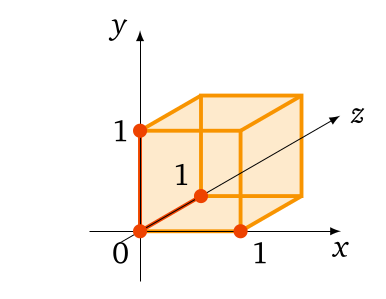
\includegraphics[width=3cm, height=3cm]{./cube.png}
   \end{itemize} 
 \end{block} 
\end{frame}

\end{document}
